%課題研究レジュメテンプレート ver. 1.2

\documentclass[uplatex]{jsarticle}
\usepackage[top=20mm,bottom=20mm,left=20mm,right=20mm]{geometry}
\usepackage[T1]{fontenc}
\usepackage{txfonts}
\usepackage{wrapfig}
\usepackage[expert,deluxe]{otf}
\usepackage[dvipdfmx,hiresbb]{graphicx}
\usepackage[dvipdfmx]{hyperref}
\usepackage{pxjahyper}
\usepackage{secdot}

\makeatletter
  \renewcommand{\section}{%
    \if@slide\clearpage\fi
    \@startsection{section}{1}{\z@}%
    {\Cvs \@plus.5\Cdp \@minus.2\Cdp}% 前アキ
    {.5\Cvs \@plus.3\Cdp}% 後アキ
    %{\normalfont\Large\headfont\raggedright}}
    {\normalfont\raggedright}}

  \renewcommand{\subsection}{\@startsection{subsection}{2}{\z@}%
    {\Cvs \@plus.5\Cdp \@minus.2\Cdp}% 前アキ
    {.5\Cvs \@plus.3\Cdp}% 後アキ
    %{\normalfont\large\headfont}}
    {\normalfont}}

  \renewcommand{\subsubsection}{\@startsection{subsubsection}{3}{\z@}%
    {\Cvs \@plus.5\Cdp \@minus.2\Cdp}%
    {\z@}%
    %{\normalfont\normalsize\headfont}}
    {\normalfont}}
\makeatother
%ここから上を編集する必要はない.

\title{\vspace{-14mm}Webサービスの障害がプロジェクトに与える影響をTwitterを活用して調査する方法}
\author{PMコース 矢吹研究室 1442012 岩瀬翔}
\date{}%日付を入れる必要はない.
\pagestyle{empty}%ページ番号は振らない.
\begin{document}
\maketitle

\section{研究の背景}
複数のメンバが同時に開発を行うソフトウェア開発プロジェクトでは,Webサービスが使われることがある.例えば,チーム内でファイルのバージョンを管理することのできる「GitHub」というサービスがある.他にもチーム内でコミュニケーションを取るためのチャットツール「Slack」やユーザレビューなどを行うために使用する「Skype」,チームで作成したファイルを共有できる「Google Drive」などがある.これらのWebサービスに障害が発生した場合,プロジェクトの進捗に影響が出るのではないかと考えた.

上記に述べた4つのWebサービスの中で,GitHubは企業においてもオープンソースソフトウェアとしてソースコードを公開するため利用されている.理由は不正なプログラムや脆弱性などの確認(監査)を行う事ができ、ソフトウェア自身の信頼性を判断する事ができるからなどである\cite{01}.そのGitHubのサーバーが2016年1月28日にダウンし,インターネット上で話題になった.実際にGitHubのサーバーダウンについて,Twitterを用いて調べてみたところ「仕事にならない」「卒論が書けない」などといった反応が多く見られた\cite{02}.

GitHubがサーバーダウンしてしまった実例から,ソフトウェア開発プロジェクト進行中にGitHubで障害が発生した場合どのような影響が生じ,その対策のために何かできることはないのかと考え研究することとした.

\section{研究の目的}
本研究の目的は次の2点を目標とする.
\begin{itemize}
 \item ソフトウェア開発プロジェクトで使用されるWebサービスに障害が発生した場合,どのような影響が発生し,その影響がどれほどの人に及ぶのか調査する.
 \item Webサービスの障害発生に対するリスク対策を考案する.
\end{itemize}
上記の目標を達成することを目的とし研究する.

\section{プロジェクトマネジメントとの関連}

本研究はプロジェクトマネジメントにおける10個の知識エリアのうち,リスクマネジメントに関連付けることができる.理由として,Webサービスの障害はソフトウェア開発プロジェクトの進捗に関わる明確なリスクだからである.

\section{研究の方法}
本研究は,ソフトウェア開発プロジェクトにおいて使用する代表的なWebサービスである,GitHubの障害発生時の状況について調査する.調査方法は,Twitterで投稿されている障害発生に関するツイートをデータとして収集する.データ収集の手順は以下の通りである\cite{03}.
\begin{enumerate}
 \item HTMLファイルからツイートの時間と本文のみを抽出するためのプログラムを作成する\cite{04}.
 \item GitHubに関連するすべてのサービスを継続的に状況監視している「GitHub Status」を参照し,2016年で障害が発生,復旧したと記録されている時間を調べる.その時間前後をTwitterで「GitHub,言語,日付,時間」を指定し検索する(例:GitHub lang:ja since:2016-10-19 until:2016-10-21\_20:30:00\_JST).その後,障害発生した旨のツイートから,復旧したという旨のツイートを表示する.
 \item 作成したプログラムをを使用して検索結果からデータを抽出する.
 \item 2~3の手順を障害発生時間ごとに繰り返す.
 \item 障害発生から復旧までの「GitHub」に対するツイート数と,どのくらいの時間で復旧が完了するのかを調べる.
 \item テキストマイニングにより頻出単語の抽出を行い,どのような影響が発生しているのか,どのような反応があるのか分析する.
 \item 分析結果を基に,リスク対策案を検討する.
\end{enumerate}


\section{現在の進捗状況}
GitHub Statusを参照に調べたところ,2016年のGitHubの障害発生回数は13回であった.発生した障害それぞれについてデータの収集を完了した.下記のグラフは,各障害の発生から復旧までに投稿されたツイートの数のグラフ,各障害の発生から復旧までの時間のグラフである.
\begin{center}
\begin{figure}[htbp]
\begin{tabular}{cc}
\begin{minipage}[t]{0.5\hsize}
 \centering
 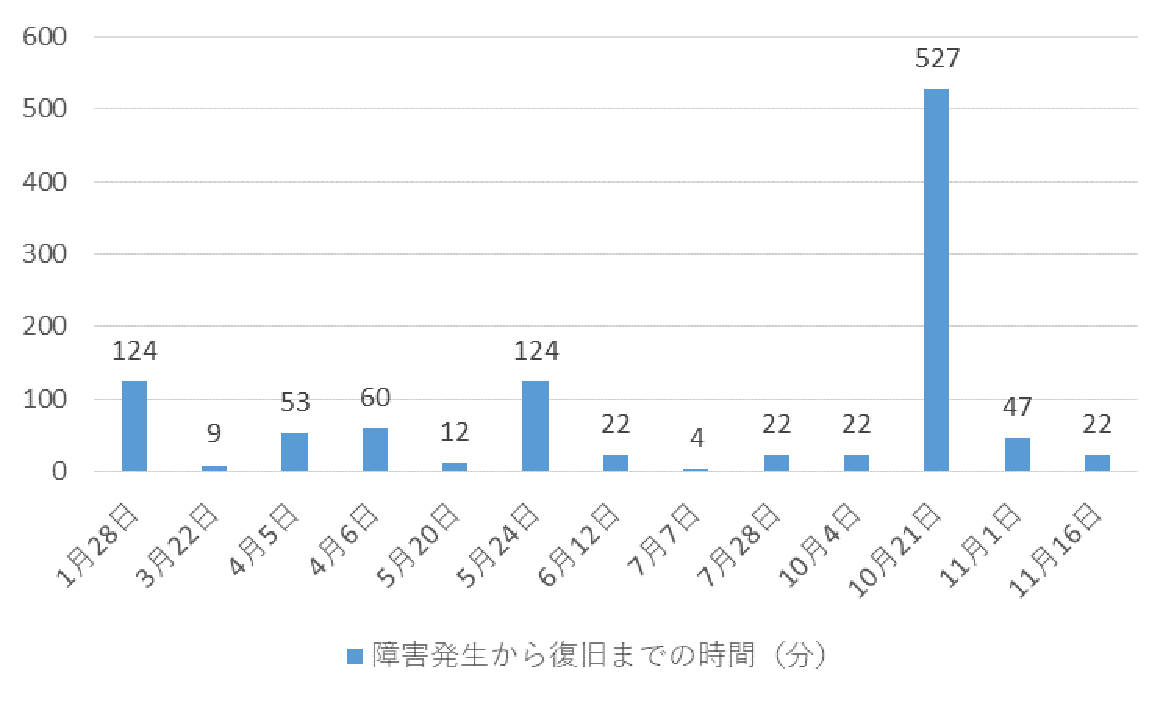
\includegraphics[width=7.5cm,clip]{graph1.pdf}
 \caption{各障害の発生から復旧までの時間}
 \label{ラベル1}
\end{minipage} &
\begin{minipage}[t]{0.5\hsize}
 \centering
 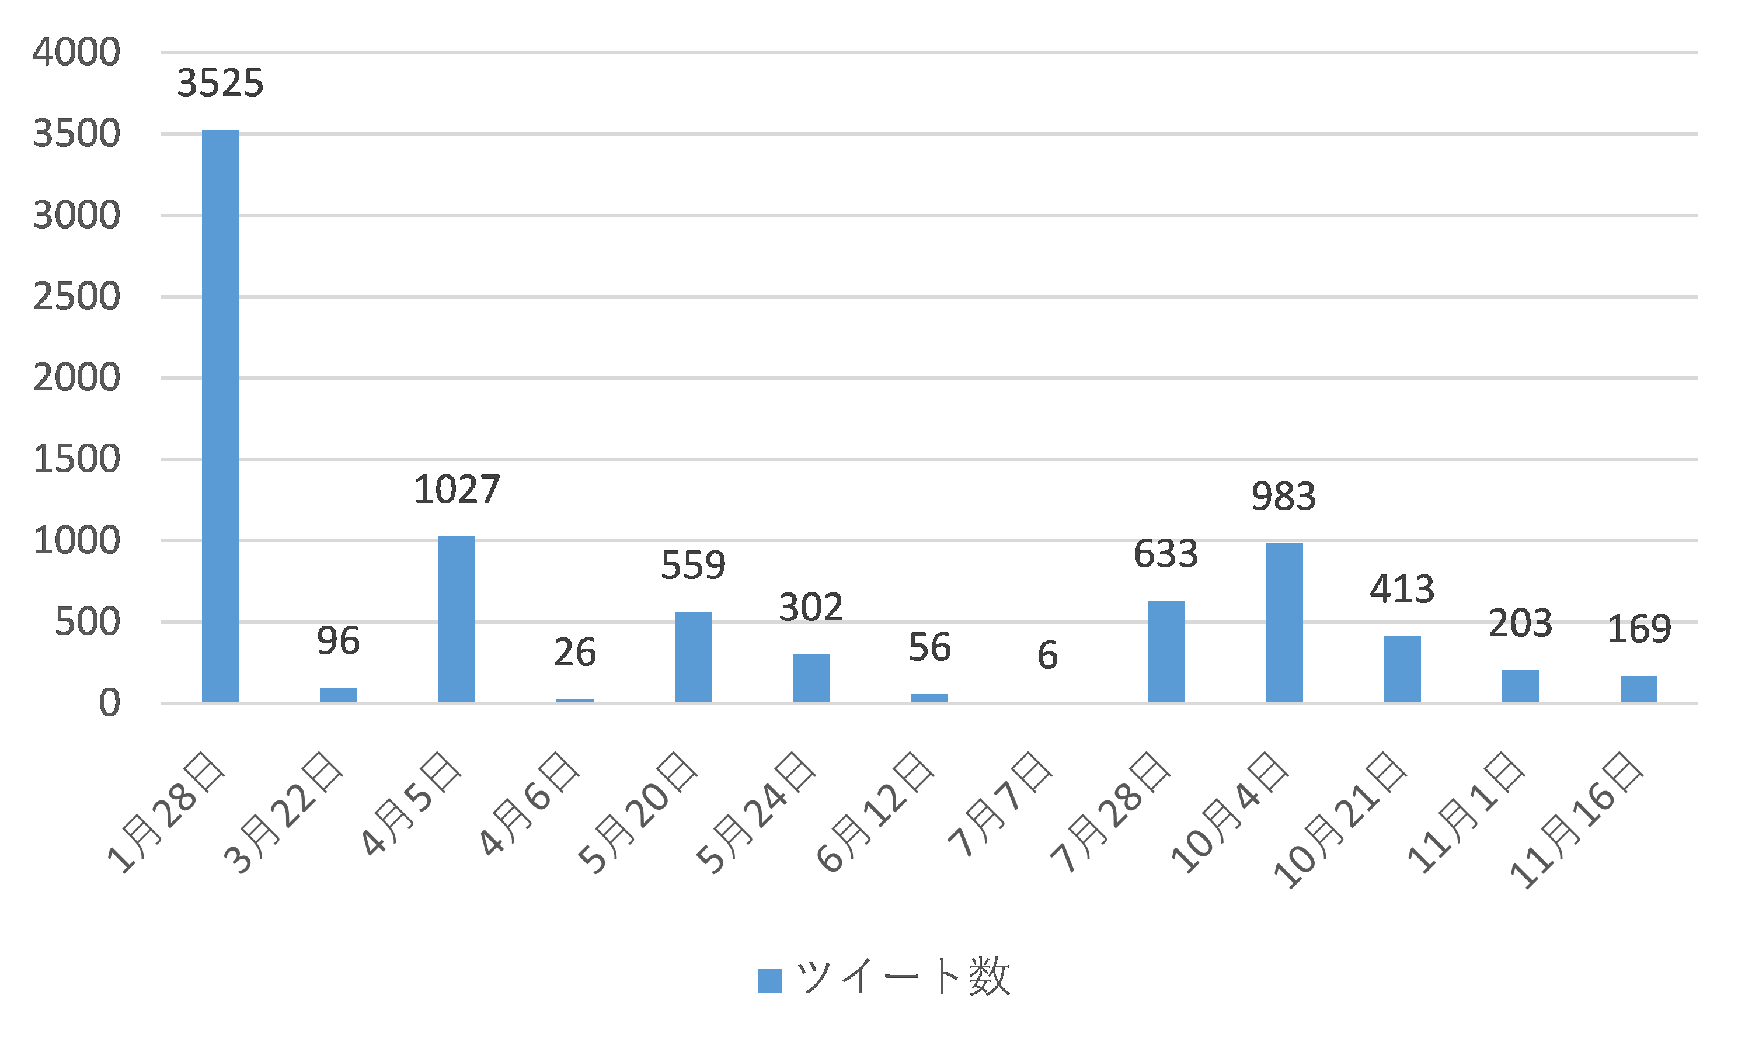
\includegraphics[width=7.5cm,clip]{graph2.pdf}
 \caption{各障害発生時のツイート数}
 \label{ラベル2}
\end{minipage}
\end{tabular}
\end{figure}
\end{center}

13回の障害を見比べてみると,障害発生の曜日,時間帯等によって取得したツイートの数に幅があることが分かった.例えば,日中の約20分間の障害でも祝日と平日では900ツイート以上の差がある.さらに,平日の日中であればツイート数が多いのはもちろんだが,深夜2時台に発生した約10分間の障害でも100件近いツイートが集まった.

また,障害の発生報告と復旧報告がGitHub Statusよりも平均約7.7分ほど速いということが分かった.

\section{今後の計画}
以下のように研究を進める計画である.
\begin{enumerate}
 \item 時間帯,曜日を加味して分析を行うことも検討する.
 \item 集めたツイート本文のデータから頻出単語を抽出し,多くツイートされている単語を分析する.
 \item 背景で述べた「Slack」「Skype」「Google Drive」の障害発生についても同様の研究する.
 \item 4つのWebサービスのデータを調査した上で,障害発生に対するリスク対策案を検討する.
\end{enumerate}

\bibliographystyle{junsrt}
\bibliography{biblio}%「biblio.bib」というファイルが必要.

\end{document}
